\section{C++ FSM Frameworks}

\subsection{FSM framework implementation}
Some basic concepts how FSM might be realized due to:

\begin{itemize}
\item Concept
    \begin{itemize}
        \item Declarative - transitions are declared at the beginning and can't be changed
        \item Imperative - transitions could have happens in custom handling on event
    \end{itemize}

\item Approach
    \begin{itemize}
        \item Compile time - transitions declared during compile time
        \item Run time - transitions declared during run time
    \end{itemize}

\item Data
    \begin{itemize}
        \item FSM driven - data in FSM
        \item State driven - data in states
        \item Action driven - data in actions
    \end{itemize}
\end{itemize}

\subsection{State machine example}
To visualize differences between frameworks small example was introduced
and implemented in all frameworks. State machine \textit{Player} contains 2 states \textit{Open and Close}.
Event \textit{OpenClose} trigger transition to the next state
(alternately \textit{Open and Close}).

\begin{figure}[htbp]
    \centering
    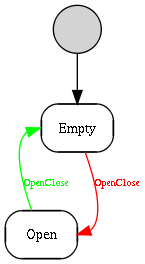
\includegraphics[scale=0.8]{images/simple.png}
    \caption[Simple state machine]{Simple state machine}
\end{figure}

\begin{enumerate}
\item \textbf{Boost Meta State Machine} (MSM)\\
\url{http://www.boost.org/doc/libs/1\_47\_0/libs/msm/doc/HTML/index.html}
\begin{itemize}
\item \textbf{Concept} Declarative
\item \textbf{Approach} Compile time
\item \textbf{Data} State driven, FSM driven
\end{itemize}
\lstinputlisting[language=C++]{frameworks/msm.hpp}

\newpage
\item \textbf{Boost State Chart} (StateChart)\\
\url{http://www.boost.org/doc/libs/1\_47\_0/libs/statechart/doc/index.html}
\begin{itemize}
\item \textbf{Concept} Declarative, Imperative
\item \textbf{Approach} Compile time, Run time
\item \textbf{Data} State driven
\end{itemize}

\lstinputlisting[language=C++]{frameworks/statechart.hpp}

\item \textbf{Quick Finite State Machine} (QFsm)
\begin{itemize}
\item \textbf{Concept} Declarative
\item \textbf{Approach} Compile time
\item \textbf{Data} Action driven
\end{itemize}
\lstinputlisting[language=C++]{frameworks/qfsm.hpp}

\end{enumerate}

